\section{Comparison with European Options}

\subsection*{Question 8: Bounding the European Put}

\textbf{Problem Statement:}
For every $x \in [0,s_0^*]$, show $v^e(0,x) \le h(x)$ and further $v^e(0,0) < h(0)$.

\textbf{Step-by-Step Solution:}
\begin{enumerate}
    \item \textbf{General Inequality:} An American option provides the same rights as a European option, plus the additional right to exercise early. Because of this added flexibility, the value of the European option can never exceed the value of the American option. Therefore, for any $x$, we have $v^e(0,x) \le v(0,x)$.
    
    \item \textbf{Applying the Early Exercise Boundary:} In Question 6, we proved that for any $x \in [0, s_0^*]$, the American option value is exactly equal to its immediate exercise value: $v(0,x) = h(x)$.
    Substituting this into our general inequality gives $v^e(0,x) \le h(x)$ for all $x \in [0, s_0^*]$.
    
    \item \textbf{Evaluating at Zero:} We must show a strict inequality at $x=0$. The initial value of the European put option is the discounted expected payoff at maturity:
    \begin{equation*}
        v^e(0,s_0) = \frac{1}{(1+r)^T} \mathbb{E}_Q[h(S_T)]
    \end{equation*}
    If the initial price is $s_0 = 0$, the asset price remains at 0 until maturity, meaning $S_T = 0$ almost surely. The payoff at maturity is therefore exactly $h(0)$.
    \begin{equation*}
        v^e(0,0) = \frac{h(0)}{(1+r)^T}
    \end{equation*}
    Because the interest rate $r > 0$, the discount factor $(1+r)^T$ is strictly greater than 1. Dividing $h(0)$ by a number strictly greater than 1 yields a result strictly less than $h(0)$. Thus, $v^e(0,0) < h(0)$.
\end{enumerate}

\subsection*{Question 9: Ordering the Exercise Boundaries}

\textbf{Problem Statement:}
Let $s_0^e := \inf\{x \in \mathbb{R}_+ : v^e(0,x) > h(x)\}$. Show $s_0^* \le s_0^e$.

\textbf{Step-by-Step Solution:}
\begin{enumerate}
    \item \textbf{Understanding the Sets:} 
    The point $s_0^*$ is the threshold where the American option value strictly exceeds the payoff: $s_0^* = \inf\{x : v(0,x) > h(x)\}$.
    The point $s_0^e$ is the analogous threshold for the European option: $s_0^e = \inf\{x : v^e(0,x) > h(x)\}$.
    
    \item \textbf{Comparing the Values:} 
    As established in Question 8, $v^e(0,x) \le v(0,x)$ for all $x$. 
    Because the European option value curve is always below or equal to the American option value curve, it takes a higher asset price for the European option to "break away" and become strictly greater than the intrinsic payoff line $h(x)$.
    
    \item \textbf{Conclusion:} Since $v(0,x)$ reaches the strict inequality condition $v(0,x) > h(x)$ before or at the same time as $v^e(0,x)$ as $x$ increases, the infimum of the American set must be less than or equal to the infimum of the European set. Hence, $s_0^* \le s_0^e$.
\end{enumerate}

\subsection*{Question 10: Option Price Graphs}

\textbf{Problem Statement:}
Draw the prices of American and European put options with respect to $s_0$.

\textbf{Visual Representation:}
Below is a graph drawn using TikZ to illustrate the relationships proven in this TD.

\begin{figure}[H]
    \centering
    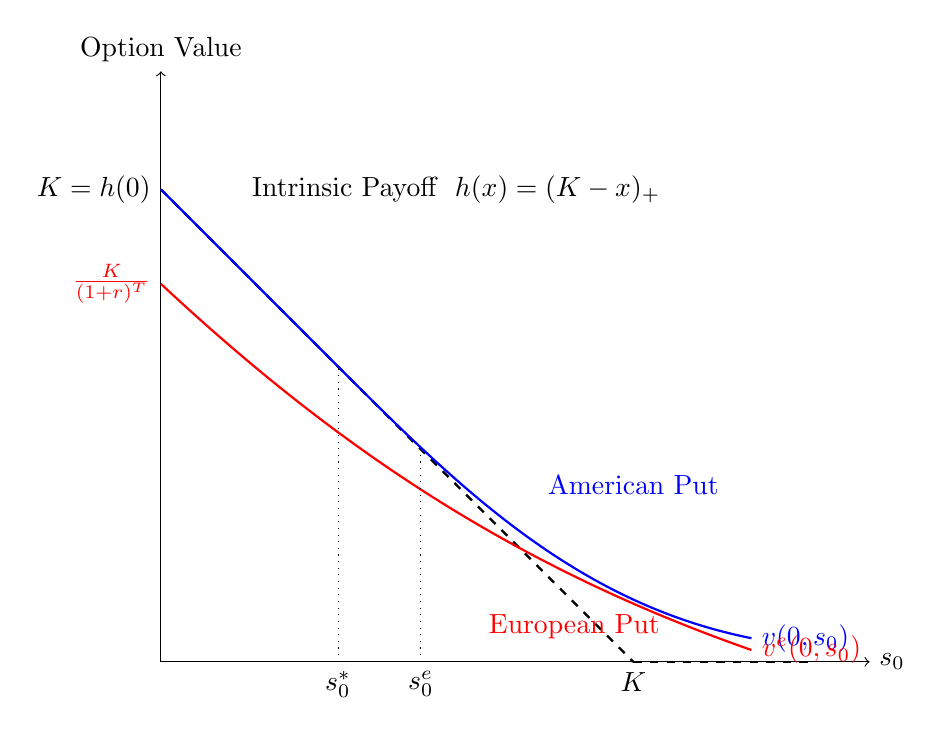
\begin{tikzpicture}[scale=1.5]
        % Axes
        \draw[->] (0,0) -- (6,0) node[right] {$s_0$};
        \draw[->] (0,0) -- (0,5) node[above] {Option Value};
        
        % Payoff function h(x)
        \draw[thick, dashed] (0,4) node[left] {$K = h(0)$} -- (4,0) node[below] {$K$};
        \draw[thick, dashed] (4,0) -- (5.5,0);
        
        % American Option v(0,x)
        \draw[thick, blue] (0,4) -- (1.5, 2.5); % matches payoff up to s_0^*
        \draw[thick, blue] (1.5, 2.5) .. controls (2.5, 1.5) and (3.5, 0.5) .. (5,0.2) node[right] {$v(0,s_0)$};
        
        % European Option v^e(0,x)
        \draw[thick, red] (0, 3.2) node[left] {$\frac{K}{(1+r)^T}$} .. controls (1.5, 1.8) and (3, 0.8) .. (5,0.1) node[right] {$v^e(0,s_0)$};
        
        % Critical points
        \draw[dotted] (1.5,0) node[below] {$s_0^*$} -- (1.5, 2.5);
        \draw[dotted] (2.2,0) node[below] {$s_0^e$} -- (2.2, 1.8);
        
        % Labels
        \node at (2.5, 4) {\text{Intrinsic Payoff } $h(x) = (K-x)_+$};
        \node[blue] at (4, 1.5) {\text{American Put}};
        \node[red] at (3.5, 0.3) {\text{European Put}};
    \end{tikzpicture}
    \caption{Prices of American and European put options with respect to the initial asset price $s_0$.}
\end{figure}